\section{Projection onto the convex sets and Dykstra's projection algorithm}

    In this section we start with the projection onto the set $C$ and go on by stating an algorithm to project onto the convex set $K$.

    \subsection{Projection onto $C$}

    The projection onto $C$ can efficiently be computed. By definition of the proximity operator we have
        $$
            u = \arg\min_{u \in C} \frac{||u-\tilde{u}||_{2}^{2}}{2} + \tau \delta_{C}(u) = \arg\min_{u \in C} \frac{||u - \tilde{u}||_{2}^{2}}{2}.
        $$
    Assume that $\tilde{u} \in C$. Then the best choice for $u$ is of course $u = \tilde{u}$ itself, since the energy  is then equal to zero, for which the quadratic function is minimal. On the other hand, if $\tilde{u} \notin C$, the euclidean distance to $C = [0, 1]$ is to clip $\tilde{u}$ onto the bound of $C$. This means if $\tilde{u} < 0$ then the shortest distance from $\tilde{u}$ to $C$ is to set $u = 0$. Reversely, if $\tilde{u} > 1$ then the euclidean distance to $C$ is given by setting $u = 1$. This idea is also illustrated in figure \ref{fig:projection_onto_c}. For an arbitrary intervall $[a, b]$ we have the following algorithm:

    \begin{algorithm}[Clipping]
        The projection of a vector $u \in \mathbb{R}^{n}$ onto the intervall $[a, b]$, where $a,b \in \mathbb{R}$ and $a < b$ is given pointwise by
            % \begin{equation}
            %     C = \{ u \in X: u(i,j,k) \in [0,1], \,\, u(i, j, 1) = 1, \,\, u(i, j, M) = 0 \}, \label{eq:limits}
            % \end{equation}
        % is given pointwise by
            \begin{equation}
                u^{n+1}_{i} = \min\{b, \max \{ a, u^{n}_{i} \} \}
                \label{ex:clipping}
            \end{equation}
        for all $i = 1, ..., n$.
    \end{algorithm}

    \begin{figure}[ht]
        \centering
        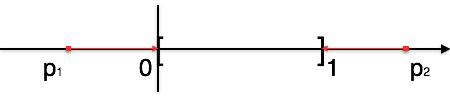
\includegraphics[width=0.9\textwidth]{img/projection_onto_c.png}
        \caption[Clipping to the set $C$]{\label{fig:projection_onto_c} A point $p_{1} < 0$ is clipped to $0$, whereas a point $p_{2} > 1$ is clipped to $1$.}
    \end{figure}

    \begin{remark}
        \begin{itemize}
            \item By projecting onto $C$, we also need to take care about the limits in \ref{eq:limits}. For that we set $u(i, j, 1) = 1$ and $u(i, j, S) = 0$ in each projection. Or similarly, using for instance the programming language C++, we have $u(i, j, 0) = 1$ and $u(i, j, S-1) = 0$.
            \item In the case of our framework - acting in a discrete cube $\mathcal{G}$ - equation \ref{ex:clipping} can be regarded as
                $$
                    u^{n+1}_{i,j,k} = \min\{1, \max \{ 0, u^{n}_{i,j,k} \} \}.
                $$
        \end{itemize}
    \end{remark}

    \subsection{The projection onto $K$} % (fold)
    \label{sub:the_projection_onto_K}

        Projecting onto $K$ is more involved than the projection onto $C$, since $K$ takes into account local and non-local constraints. In other words, the set $K$ is an intersection of several convex sets. The projection onto the intersection of convex sets can be done by Dykstra's projection algorithm. The idea behind this algorithm is to project onto each set alternatingly in a step $n$ and store the error, which is made in this iteration step. Before the projection in the $n+1$-th step is done, the vector which should be projected is reduced by the error made in the previous step. To fully understand this scheme, we first give the definition which was first proposed by Boyle and Dykstra in \cite{dykstra-et-al-aors14}, where one can also find a proof of convergence. Afterwards, we will provide and discuss the algorithm and additionally show an example.

        \begin{algorithm}
        \label{alg:dykstra}
            Consider $P$ convex sets with $\mathbb{R}^{n} \ni X = X_{1} \cap X_{2} \cap ... \cap X_{P}$. Let $\Pi_{i}$ denote the projection onto the i-th set for $i = 1, ..., P$. And let $u_{c} \in \mathbb{R}^{n}$ be the current estimate with $u_{c} \notin X$, $u_{i}^{k} \in \mathbb{R}^{n}$ for $i = 0, ..., P$ and $v_{i}^{k} \in \mathbb{R}^{n}$ for $i = 1, ..., P$ and $k = 1, 2, ...$, where $k$ denotes the number of iterations. Then the algorithm finds the (only) $u^{\ast} \in X$, such that

            $$
                ||u^{\ast} - u_{c}||^{2} \le ||u - u_{c}||^{2} \,\,\, \forall u \in X.
            $$

            For $k = 1, 2, ...$ set $u^{0}_{P} = u_{c}$ and $v^{0}_{i} = 0$ for all $i = 1, ..., P$. Then iterate until convergence (e.g. $||u_{0}^{k} - u_{P}^{k}||_{2} \le \varepsilon$ with $\varepsilon$ small):

            \begin{eqnarray}
                &u_{0}^{k} = &u_{P}^{k-1}, \notag \\
                &\textnormal{for} \,\, &i = 1, 2, ..., P: \notag \\
                &&u_{i}^{k} = \Pi_{i}(u_{i-1}^{k} - v_{i}^{k-1}), \notag \\
                &&v_{i}^{k} = u_{i}^{k} - (u_{i-1}^{k} - v_{i}^{k-1}). \notag
            \end{eqnarray}
        \end{algorithm}

        \begin{theorem}[Convergence]
            The sequence $u_{0}^{k}$ in algorithm \ref{alg:dykstra} converges to the (only) point $u \in X$.
        \end{theorem}
        As mentioned, the proof for the theorem can be found in \cite{dykstra-et-al-aors14}.

        % Recalling algorithm \ref{alg:dykstra}, we see that in each iteration step $k$ we project the current vector $u_{i-1}^{k}$ minus the error we made in the previous step, onto the i-th set. Afterwards, we update the error vector $v_{i}^{k}$. As illustrated in (BILD!!!), we project alternatingly on each set. At the end we convergence to the (only) point in $K$.

        Now, that we know how the projection onto the entire set $K$ can be implemented, we need to discuss how a projection onto the subsets of $K$ can be computed. First let us give a decomposition of $K$ into two several sets.
    % subsection the_projection_onto_K (end)

    \subsection{Decomposition of $K$} % (fold)
    \label{sub:decomposition_of_K}
        
        We will decompose the set $K$ into sets $K_{p}$ and $K_{nl}$, where the first resembles the local constraint, or more precisely, a parabola constraint and the second corresponds to the non-local constraint. Overall, we have $K = K_{p} \cap K_{nl}$ with

    \begin{equation}
        % &K_{p}& = \bigg\{ p^{3}(i,j,k) \ge \frac{p^{1}(i,j,k)^{2} + p^{2}(i,j,k)^{2}}{4} - \lambda(\frac{k}{M} - f(i,j))^{2} \bigg\} \,\,\, \forall i, j, k \notag \\
        K_{p} = \bigg\{ p^{t}(i, j, k) \ge \frac{||p^{x}(i, j, k)||^{2}}{4} - \lambda(\frac{k}{M} - f(i,j))^{2} \bigg\} \,\,\, \forall i, j, k \label{eq:parabola}
        % \Longleftrightarrow &K_{p}& = \bigg\{ p^{t}(i, j, k) \ge \frac{||p^{x}(i, j, k)||^{2}}{4} - \lambda(\frac{k}{M} - f(i,j))^{2} \bigg\} \,\,\, \forall i, j, k \label{eq:parabola}
    \end{equation}

    where $p^{t}(i, j, k) = p^{3}(i, j, k)$ and $p^{x}(i, j, k) = (p^{1}(i, j, k), p^{2}(i, j, k))^{T}$. For the non-local constraint we have

    \begin{equation}
        K_{nl} = \bigg\{ \left| \sum_{k_{1} \le k \le k_{2}} p^{x}(i, j, k) \right| \le \nu \bigg\} \,\,\, \forall i, j, k_{1} \le k \le k_{2}. \label{eq:nonlocal}
    \end{equation}

    We will now deduce the projection on these two sets. Let us start with the projection onto the parabola.
    %Since $K_{p}$ is an intersection of $P \cdot N \cdot M$ set and $K_{nl}$ is an intersection of $P \cdot N \cdot (\frac{M(M-1)}{2} + M)$ sets we need an algorithm which can handle the projection of a point onto (convex) sets. First let us introduce the projections onto $K_{p}$ and $K_{nl}$.

    % subsection decomposition_of_K (end)

    \subsection{Projection onto $K_{p}$}

        Since the projection onto the set $K_{p}$ is pointwise we want to drop the indices $(i, j, k)$. Note that we do not necessarily need that a $p^{x}$ is an element of $\mathbb{R}^{2}$. The following derivation holds for a larger class of problems namely having $p^{x} \in \mathbb{R}^{n}$. Let $\alpha > 0$, $p^{x} \in \mathbb{R}^{n}$, $p^{t} \in \mathbb{R}$ and $p = (p^{x}, p^{t})^{T} \in \mathbb{R}^{n} \times \mathbb{R}$. Assume that $p_{0}^{t} < \alpha ||p_{0}^{x}||_{2}^{2}$ holds for a point $p_{0} \in \mathbb{R}^{n}\times\mathbb{R}$. Then the projection of $p_{0}$ onto the parabola $\alpha ||p_{0}^{x}||_{2}^{2}$ can be written as the following minimization problem

            \begin{eqnarray}
                &\min\limits_{p \in \mathbb{R}^{n} \times \mathbb{R}}& \frac{1}{2} ||p - p_{0}||_{2}^{2} \notag \\
                &\textnormal{subject to}& p^{t} \ge \alpha||p^{x}||_{2}^{2} \notag
            \end{eqnarray}

        % Defining $f(p) = \frac{(p - p_{0})^{2}}{2}$ and $g(p) = p^{t} - \alpha ||p^{x}||_{2}^{2}$ the above convex optimization problem is equivalent to

        %     \begin{eqnarray}
        %         &\min\limits_{p \in \mathbb{R}^{n} \times \mathbb{R}}& f(p) \notag \\
        %         &\textnormal{subject to}& g(p) \ge 0 \notag
        %     \end{eqnarray}

        To find the solution of this optimization problem we introduce a Lagrange Multiplier $\mu \in \mathbb{R}$ and define the Lagrangian as

        \begin{equation}
            \mathcal{L}(p, \mu) = \frac{(p - p_{0})^{2}}{2} - \mu \bigg( p^{t} - \alpha||p^{x}||_{2}^{2} \bigg).
        \end{equation}

        We are seeking to minimize $\mathcal{L}(p, \mu)$ over all $p$ and $\mu$. The minimization problem we consider is convex, because our function to optimize is convex, the inequality constraint is convex and the feasible set $\mathbb{R}^{n} \times \mathbb{R}$ is also convex. For that, we know that computing a critical point of the Lagrangian function $\mathcal{L}$ also leads to a global optimum of the optimization problem itself. We compute a critical point with
        % Setting $\nabla \mathcal{L}(p, \mu) = 0$ we derive a global minimum, since our function to optimize is convex, the inequality constraint is convex and the feasible set $\mathbb{R}^{n} \times \mathbb{R}$ is also convex. We set

        \begin{equation}
            \nabla \mathcal{L}(p, \mu) =
            \begin{pmatrix}
                \partial_{p^{x}} \mathcal{L}(p, \mu) \\
                \partial_{p^{t}} \mathcal{L}(p, \mu) \\
                \partial_{\mu} \mathcal{L}(p, \mu)
            \end{pmatrix} = 
            \begin{pmatrix}
                p^{x} - p_{0}^{x} + \mu 2 \alpha p^{x} \\
                p^{t} - p_{0}^{t} - \mu \\
                p^{t} - \alpha||p^{x}||_{2}^{2}
            \end{pmatrix}
            = 0. \label{eq:linearSystem}
        \end{equation}

        That means, we need to solve a linear system. The first equation gives us

        \begin{equation}
            p_{0}^{x} = (\mu 2 \alpha + 1) p^{x} \Longleftrightarrow p^{x} = \frac{p_{0}^{x}}{\mu 2 \alpha + 1}, \label{eq:1stequ}
        \end{equation}

        and the second equation leads us to

        \begin{equation}
            p^{t} = p_{0}^{t} + \mu. \label{eq:2ndequ}
        \end{equation}

        % We can solve this system in two ways:
        In the following we discuss two different possibilities how the system \ref{eq:linearSystem} can be solved.
        \begin{enumerate}
            \item Plugging the equalities \ref{eq:1stequ} and \ref{eq:2ndequ} into the third line of equation \ref{eq:linearSystem}, we get

        \begin{eqnarray}
            p^{t} - \alpha||p^{x}||_{2}^{2} &\Longleftrightarrow& p_{0}^{t} + \mu - \alpha \bigg|\bigg|\frac{p_{0}^{x}}{\mu 2 \alpha + 1}\bigg|\bigg|_{2}^{2} = 0 \Longleftrightarrow p_{0}^{t} + \mu - \frac{\alpha}{(\mu 2 \alpha + 1)^{2}} ||p_{0}^{x}||_{2}^{2} = 0 \notag \\
            &\overbrace{\Longleftrightarrow}^{\cdot (\mu2\alpha + 1)^{2}}& (\mu 2 \alpha + 1)^{2} p_{0}^{t} + (\mu 2 \alpha + 1)^{2} \mu - \alpha ||p_{0}^{x}||_{2}^{2} = 0 \notag \\
            &\Longleftrightarrow& (4 \mu^{2} \alpha^{2} + 4 \mu \alpha + 1) p_{0}^{t} + 4 \mu^{3} \alpha^{2} + 4 \mu^{2} \alpha + \mu - \alpha ||p_{0}^{x}||_{2}^{2} = 0 \notag \\
            &\Longleftrightarrow& 4 \alpha^{2} \mu^{3} + \mu^{2} (4 \alpha^{2} p_{0}^{t} + 4 \alpha) + \mu (4 \alpha p_{0}^{t} + 1) + p_{0}^{t} - \alpha ||p_{0}^{x}||_{2}^{2} = 0. \notag
        \end{eqnarray}

        Defining a function
            $$
                h(\mu) = 4 \alpha^{2} \mu^{3} + \mu^{2} (4 \alpha^{2} p_{0}^{t} + 4 \alpha) + \mu (4 \alpha p_{0}^{t} + 1) + p_{0}^{t} - \alpha ||p_{0}^{x}||_{2}^{2},
            $$
        we are seeking for the zeroes of $h$. Computing the zeroes can efficiently be established by using Newton's algorithm defined by

        \begin{equation}
            \mu^{k+1} = \mu^{k} - \frac{h(\mu)}{h^{'}(\mu)}, \label{eq:newton}
        \end{equation}

        for $k = 1, 2, ...$.

        If we set
        $$
            h(\mu) = 4 \alpha^{2} \mu^{3} + \mu^{2} (4 \alpha^{2} p_{0}^{t} + 4 \alpha) + \mu(4 \alpha p_{0}^{t} + 1) + p_{0}^{t} - \alpha ||p_{0}^{x}||_{2}^{2},
        $$
        the first derivative of $h$ is given by
        $$
            h^{'}(\mu) = 12 \alpha^{2} \mu^{2} + 2 \mu (4 \alpha^{2} p_{0}^{t} + 4 \alpha) + (4 \alpha p_{0}^{t} + 1).
        $$
        Overall, we get the update equation for a $\mu^{k+1}$ with
            \begin{equation}
                \mu^{k+1} = \mu^{k} - \frac{4 \alpha^{2} \mu^{3} + \mu^{2} (4 \alpha^{2} p_{0}^{t} + 4 \alpha) + \mu(4 \alpha p_{0}^{t} + 1) + p_{0}^{t} - \alpha ||p_{0}^{x}||_{2}^{2}}{12 \alpha^{2} \mu^{2} + 2 \mu (4 \alpha^{2} p_{0}^{t} + 4 \alpha) + (4 \alpha p_{0}^{t} + 1)}.
            \end{equation}
        In \cite{Chambolle-et-al-10} they suggest setting $\mu^{0} = \max \{ 0, - \frac{2 p_{0}^{t}}{3} \}$, where they state that Newton's method converges within 7-10 iterations to a quite accurate solution.\\
        The projected vector $p$ of our problem is then given by
            \begin{equation}
                p = \bigg( \frac{p_{0}^{x}}{\mu 2 \alpha + 1}, p_{0}^{t} + \mu \bigg), \label{eq:newtonSolution}
            \end{equation}
        which we get from equations \ref{eq:1stequ} and \ref{eq:2ndequ}. We did not apply this method to our framework, since the primal-dual algorithm will be extremley slow in the case of this framework. Having a few iterations of Newton's algorithm in each iteration step would generate more overhead and for that would decelerate the program. Further, Newton's method is inexact and as it turns out, the second approach to this problem will lead to an exact solution, which can be computed within one loop of straightforward computations.

        \item For the second approach we note that \ref{eq:1stequ} and \ref{eq:2ndequ} hold and the third equation in \ref{eq:linearSystem} can be expressed with
        \begin{equation}
            p^{t} = \alpha ||p^{x}||_{2}^{2} \Longleftrightarrow \alpha ||p^{x}||_{2}^{2} = \underbrace{p_{0}^{t} + \mu}_{p^{t}}. \label{eq:tmp1}
        \end{equation}
        With equation \ref{eq:1stequ} we can also compute the solution of $\mu$ by using that

        \begin{eqnarray}
            p^{x} = \frac{p_{0}^{x}}{\mu 2 \alpha + 1} &\Longleftrightarrow& ||p^{x}||_{2} = \bigg|\bigg| \frac{p_{0}^{x}}{1 + 2 \alpha \mu} \bigg|\bigg|_{2} \Longleftrightarrow ||p^{x}||_{2} = \frac{1}{1 + 2 \alpha \mu} ||p_{0}^{x}||_{2} \notag \\
            &\Longleftrightarrow& \frac{1}{1 + 2 \alpha \mu} = \frac{||p^{x}||_{2}}{||p_{0}^{x}||_{2}} \notag \\
            &\Longleftrightarrow& 1 + 2\alpha\mu = \frac{||p_{0}||_{2}}{||p_{x}||_{2}} \notag \\
            &\Longleftrightarrow& 2 \alpha \mu = \frac{||p_{0}^{x}||_{2}}{||p^{x}||_{2}} - 1 \notag \\
            &\Longleftrightarrow& \mu = \frac{1}{2 \alpha} \bigg( \frac{||p_{0}^{x}||_{2}}{||p^{x}||_{2}} \bigg) - \frac{1}{2\alpha}. \notag
        \end{eqnarray}

        Using the solution of $\mu$ in \ref{eq:tmp1} we get

        \begin{eqnarray}
            \alpha ||p^{x}||_{2}^{2} = p_{0}^{t} + \frac{1}{2 \alpha} \bigg( \frac{||p_{0}^{x}||_{2}}{||p^{x}||_{2}} \bigg) - \frac{1}{2\alpha} &\overbrace{\Longleftrightarrow}^{\cdot 2 \alpha ||p^{x}||_{2}}& 2 \alpha^{2} ||p^{x}||_{2}^{3} = 2 \alpha ||p^{x}||_{2} p_{0}^{t} + ||p_{0}^{x}||_{2} - ||p^{x}||_{2} \notag \\
            &\Longleftrightarrow& 2 \alpha^{2} ||p^{x}||_{2}^{3} + 2\alpha||p^{x}||_{2} - 2\alpha p_{0}^{t} ||p^{x}||_{2} - ||p_{0}^{x}||_{2} = 0. \notag \\
            &\Longleftrightarrow& 2 \alpha^{2} ||p^{x}||_{2}^{3} + (1 - 2 \alpha p_{0}^{t}) ||p^{x}||_{2} - ||p_{0}^{x}||_{2} = 0. \notag \\
            &\overbrace{\Longleftrightarrow}^{\cdot 4 \alpha}& 8 \alpha^{3} ||p^{x}||_{2}^{3} + 4 \alpha (1 - 2 \alpha p_{0}^{t}) ||p^{x}||_{2} - 4 \alpha ||p_{0}^{x}||_{2} = 0. \notag \\
            &\Longleftrightarrow& (2 \alpha ||p^{x}||_{2})^{3} + 2 (1 - 2 \alpha p_{0}^{t}) 2 \alpha ||p^{x}||_{2} - 4 \alpha ||p_{0}^{x}||_{2} = 0. \notag \\
            &\Longleftrightarrow& t^{3} + 3bt - 2a = 0, \label{eq:cubic}
        \end{eqnarray}

        with $a = 2 \alpha ||p_{0}^{x}||_{2}$, $b = \frac{2}{3}(1 - 2 \alpha p_{0}^{t})$ and $t = 2 \alpha ||p^{x}||_{2}$.\\
        The cubic equation \ref{eq:cubic} in $t$ can efficiently be solved using the analytical formula for solving cubic equation published by J. P. McKelvey in 1984 in \cite{kelvey-ajp}.

        \end{enumerate}

        The result of the work mentioned is summarized in the following algorithm. Notice that we already computed the factors $a$ and $b$. The others follow with \cite{kelvey-ajp}.

            \begin{algorithm}

                If already $p_{0}^{t} \ge \alpha ||p_{0}^{x}||_{2}^{2}$, the solution is $(p^{x}, p^{t}) = (p_{0}^{x}, p_{0}^{t})$. Otherwise, with $a = 2 \alpha ||p_{0}^{x}||_{2}$, $b = \frac{2}{3} (1 - 2 \alpha p_{0}^{t})$, and

                    \[
                        d =
                            \begin{dcases*}
                                a^{2} + b^{3} & \textnormal{if $b \ge 0$}\\
                                (a - \sqrt{-b}^{3})(a + \sqrt{-b}^{3}) & \textnormal{else}
                            \end{dcases*}
                    \]

                set

                    \[
                        v =
                            \begin{dcases*}
                                c - \frac{b}{c} \,\, \textnormal{with} \,\, c = \sqrt[3]{a + \sqrt{d}} & \textnormal{if $d \ge 0$}\\
                                2 \sqrt{-b} \cos \bigg( \frac{1}{3} \arccos \frac{a}{\sqrt{-b}^{3}} \bigg) & \textnormal{else}.
                            \end{dcases*}
                    \]

                If $c = 0$ in the first case, set $v = 0$. The solution is then given by

                    \[
                        p^{x} =
                            \begin{dcases*}
                                \frac{v}{2\alpha} \frac{p_{0}^{x}}{||p_{0}^{x}||_{2}} & \textnormal{if $p_{0}^{x} \ne 0$}\\
                                0 & \textnormal{else}
                            \end{dcases*}
                    \]

                and $p^{t} = \alpha ||p^{x}||_{2}^{2}$.
            \end{algorithm}

        The above method states that the projection onto the parabola can be done by one cycle of straightforward computations. The implementation of it is quite simple and computation time is fast. Compared to Newton's algorithm, which is inexact, we get a exact solution and save a huge amount of run-time.

    \subsection{Projection onto $K_{nl}$}

        This set is a combination of non-local constraints, meaning that in a fixed point $(i, j, k)$ we sum up for all possible combinations $k_{1} \le k \le k_{2}$ for all $k, k_{1}, k_{2} = 1, ..., S$. For that reason you can not project pointwise. Let us first present the algorithm:

        \begin{algorithm}[Soft Shrinkage Scheme]
        \label{alg:softshrinkage}
            Let $p^{i}_{k} = (p^{1}(i, j, k), p^{2}(i, j, k))^{T} \in \mathbb{R}^{2}$, $p^{i} = (p^{i}_{1}, ..., p^{i}_{S})^{T} \in \mathbb{R}^{2 \times S}$ for all $i = 1, 2, ...$. Then the projection $p^{n+1}$ of a $p^{n}$ - for an arbitrary, fixed pair $(k_{1}, k_{2})$ with $1 \le k_{1} \le k \le k_{2} \le S$ - is computed by:

                \[
                    p^{n+1} =
                        \begin{dcases*}
                            p^{n} + \frac{s - \tilde{s}}{k_{2} - k_{1} + 1} & \textnormal{if $k_{1} \le k \le k_{2}$}, \\
                            p^{n} & \textnormal{else},
                        \end{dcases*}
                \]

            where $s \in \mathbb{R}^{2}, \tilde{s} \in \mathbb{R}^{2}$ with

                $$\tilde{s} = \sum_{k_{1} \le k \le k_{2}} p^{n}_{k}$$

            and

                \[
                    s =
                        \begin{dcases*}
                            \tilde{s} & \textnormal{if $||\tilde{s}||_{2} \le \nu$},\\
                            \Pi_{||\cdot||_{2} \le \nu}(\tilde{s}) = \frac{\nu}{||\tilde{s}||_{2}} \tilde{s} & \textnormal{else}.
                        \end{dcases*}
                \]

        \end{algorithm}

        Since this procedure needs a clarification, we need the KKT conditions. Following the notation, definition and theorem of \cite{Nocedal-Wright}, we consider the optimization problem:

            \begin{equation}
                \min_{x \in \mathbb{R}^{n}} \, f(x) \,\,\,\,\, \textnormal{subject to} \,\,\,
                \begin{dcases*}
                    c_{i}(x) = 0 & $i \in \mathcal{E}$, \\
                    c_{i}(x) \ge 0 & $i \in \mathcal{I}$,
                \end{dcases*}
                \label{eq:basic_optimization_problem}
            \end{equation}
        where $f$ and for all $i \in \mathcal{E} \cup \mathcal{I}$ the functions $c_{i}$ are smooth, real-valued functions on a subset of $\mathbb{R}^{n}$. Further, $\mathcal{E}$ and $\mathcal{I}$ denote two finite sets of indices. Here, $f$ is the objective function, whereas the $c_{i}$ for $i \in \mathcal{E}$ are the equality constraints and $c_{i}$ with $i \in \mathcal{I}$ the inequality constraints. We further want to define the feasible set $\Omega$. As stated in section \ref{sec:convex_optimization_and_convex_analysis} this set is the set of all points, which satisfy the constraints $c_{i}$ for all $i$. Then we have
            \begin{equation}
                \Omega = \{ x \,\, | \,\, c_{i}(x) = 0, \,\, i \in \mathcal{E}; \,\, c_{i} \ge 0, \,\, i \in \mathcal{I} \}.
                \label{eq:feasible_set_omega}
            \end{equation}
        We rewrite our optimization problem in terms of the set $\Omega$ to
            $$
                \min_{x \in \Omega} f(x).
            $$

        Additionally, we want to define the so called active set for the constraint functions.

        \begin{definition}[Active Set]
            \label{def:active_set}
            The active set $\mathcal{A}(x)$ at any feasible $x$ consists of the equality constraint indices from $\mathcal{E}$ together with the indices of the inequality constraints $i$, for which $c_{i}(x) = 0$, that is
                \begin{equation}
                    \mathcal{A}(x) = \mathcal{E} \cup \{ i \in \mathcal{I} | c_{i}(x) = 0 \}
                    \label{eq:active_set}
                \end{equation}
        \end{definition}

        We call a inequality constraint active if $c_{i} = 0$ and inactive if $c_{i} > 0$, for a $i \in \mathcal{I}$. The definition of the active set is an important basis for the following definition.

        \begin{definition}[LICQ]
            \label{def:licq}
            Given the point $x$ and the active set $\mathcal{A}(x)$, we say that the linear independence constraint qualification (LICQ) holds if the set of active constraint gradients
                $$
                    \{ \nabla c_{i}(x), \, i \in \mathcal{A}(x) \}
                $$
            is linearly independent.
        \end{definition}

        Then, we can propose the first-order necessary conditions, which are also well known as the Karush-Kuhn-Tucker (KKT) optimality conditions.

        \begin{theorem}[Karush-Kuhn-Tucker Optimality Conditions]
        \label{the:kkt_conditions}
            Suppose that $x^{\ast}$ is a local solution of equation \ref{eq:basic_optimization_problem}, that the
            functions $f$ and $c_{i}$ are continuously differentiable, and that the LICQ holds at $x^{\ast}$. Then there is a Lagrange multiplier vector $\lambda^{\ast}$, with components $\lambda_{i}^{\ast}, i \in \mathcal{E} \cup \mathcal{I}$, such that the following conditions are satisfied at $(x^{\ast}, \lambda^{\ast})$.
            \begin{subequations}
                \begin{align}
                    \nabla_{x}\mathcal{L}(x^{\ast}, \lambda^{\ast}) &= 0, \label{eq:stationarity} \\
                    c_{i}(x^{\ast}) &= 0, \,\,\,\,\, \textnormal{for all} \, i \in \mathcal{E}, \\
                    c_{i}(x^{\ast}) &\ge 0, \,\,\,\,\, \textnormal{for all} \, i \in \mathcal{I}, \\
                    \lambda_{i}^{\ast} &\ge 0, \,\,\,\,\, \textnormal{for all} \, i \in \mathcal{I}, \\
                    \lambda_{i}^{\ast}c_{i}(x^{\ast}) &= 0, \,\,\,\,\, \textnormal{for all} \, i \in \mathcal{E} \cup \mathcal{I}.\label{eq:complementary_conditions}
                \end{align}
                \label{eq:kkt_conditions}
            \end{subequations}
        \end{theorem}

        \begin{remark}
            The last condition \ref{eq:complementary_conditions} in the theorem is also known as the complementary slackness condition. It implies that either the $i$-th constraint is active or $\lambda_{i}^{\ast} = 0$. It is also possible, that both are zero.
        \end{remark}

    A proof of theorem \ref{the:kkt_conditions} can, for instance, be found in \cite{Nocedal-Wright}. Let us now proof, that the algorithm \ref{alg:softshrinkage} is valid, by using the KKT conditions.

    \begin{proof}
        Let $\tilde{s}, s, p_{k}, \tilde{p}_{k} \in \mathbb{R}^{2}$ and $p, \tilde{p} \in \mathbb{R}^{2 \times M}$ have the same form as in algorithm \ref{alg:softshrinkage}. For a fixed pair $(k_{1}, k_{2})$ we face the following optimization problem:

        \begin{subequations}
            \begin{align}
            \min\limits_{p \in \mathbb{R}^{2 \times M}} &\frac{1}{2} ||p - \tilde{p}||^{2}_{2} \\
            \textnormal{subject to} \,\,\, &\bigg{|} \bigg{|} \sum_{k_{1} \le k \le k_{2}} p_{k} \bigg{|} \bigg{|}_{2} \le \nu. \label{eq:inequalityConstraint}
            \end{align}
            \label{eq:optimization_problem}
        \end{subequations}

        The problem states that we try to find the closest $p$ to $\tilde{p}$ whose components fullfil the inequality constraint in \ref{eq:inequalityConstraint}, which can also be written as
            $$
                \bigg{|} \bigg{|} \sum_{k_{1} \le k \le k_{2}} p_{k} \bigg{|} \bigg{|}_{2} - \nu \le 0.
            $$

        % If we define functions
        %     $$
        %         f(p) = \sum_{k = 1}^{M} \frac{(p_{k} - \tilde{p}_{k})^{2}}{2}, \,\,\,\,\, g_{i}(p) = \frac{1}{2} \nu^{2} - \frac{1}{2} ||\tilde{s}||_{2}^{2} \tilde{s}
        %     $$
        % for i = 1, then an equivalent formulation of the system \ref{eq:optimization_problem} would be
        % \begin{subequations}
        %     \begin{align}
        %         &\min\limits_{p \in \mathbb{R}^{2 \times M}} &f(p) \\
        %         &\textnormal{subject to} &g_{i}(p) \ge 0,
        %     \end{align}
        %     \label{eq:problem_to_solve}
        % \end{subequations}

        % with the set of indices $\mathcal{I} = \{1\}$. Note, that we have no equality constraints in this optimization problem. Since this optimization problem only has one constraint, we drop the index for the function $g$ in the following. %Since the function $g(p)$ for a fixed pair $(k_{1}, k_{2})$ is a real-valued function, the active set for this problem is
            % $$
            %     \mathcal{A}(x) = \{ i \in \mathcal{I} \, | \, g_{i}(p) = 0 \}.
            % $$
        % With this we want to show, that the LICQ definition is fullfild. For this let us compute
        %     \begin{eqnarray}
        %         \{ \nabla g_{i}(x), \, i \in \mathcal{A}(x) \} &=& \bigg\{ \nabla \bigg( \frac{1}{2} \nu^{2} - \frac{1}{2} \bigg{|} \bigg{|} \sum_{k_{1} \le k \le k_{2}} p_{k} \bigg{|} \bigg{|}_{2}^{2} \bigg) \bigg\} \notag \\
        %         &=& \bigg\{ - \sum_{k_{1} \le k \le k_{2}} p_{k} \bigg\} \notag \\
        %         &=& \{-\tilde{s}\} \notag
        %     \end{eqnarray}

        The feasible set for a point $(k_{1}, k_{2})$ of this optimization problem is given by
            $$
                \mathcal{F}_{p} = \{ p \in Y \, | \, \sum_{k_{1} \le k \le k_{2}} p_{k} \,\, \forall \, k_{1} \le k \le k_{2} \, \textnormal{with} \, k = 1, ..., S \}.
            $$
        If $\tilde{p} \in \mathcal{F}_{p}$, the inequality constraint is fullfild and for that $p = \tilde{p}$ leads to the minimal energy, which is zero. For that reason, we only consider points $\tilde{p} \notin \mathcal{F}_{p}$.

        %Clearly, $\tilde{s}$ is, linearly independent (of itself) and we can make use of the KKT conditions.
        Let us introduce a Lagrange multiplier variable $\lambda \in \mathbb{R}$ and observe the Lagrange function
        \begin{equation}
            \mathcal{L}(p, \lambda) = f(p) - \lambda g(p) = \sum_{k = 1}^{M} \frac{(p_{k} - \tilde{p}_{k})^{2}}{2} - \lambda \frac{1}{2} \nu^{2} - \frac{1}{2} - \bigg{|} \bigg{|} \sum_{k_{1} \le k \le k_{2}} p_{k} \bigg{|} \bigg{|}_{2}.
        \end{equation}

        Considering equation \ref{eq:stationarity} and assume that $p^{\ast}_{k} = \tilde{p}_{k} + \frac{s - \tilde{s}}{k_{2} - k_{1} + 1}$ is a feasible point, that satisfies LICQ and is a local solution of system \ref{eq:optimization_problem}, together with a optimal $\lambda^{\ast}$. Then we have

        \begin{equation}
            \nabla_{p} \mathcal{L}(p^{\ast}, \lambda^{\ast}) = \nabla_{p} f(p^{\ast}) + \lambda \nabla_{p} g(p^{\ast}) =
            \underbrace{\begin{pmatrix}
                p^{\ast}_{1} - \tilde{p}_{1} \\
                 \\
                \vdots \\
                 \\
                \vdots \\
                 \\
                \vdots \\
                 \\
                p^{\ast}_{S} - \tilde{p}_{S}
            \end{pmatrix}}_{\in \mathbb{R}^{S}}
            + \lambda^{\ast}
            \underbrace{\begin{pmatrix}
                0 \\
                \vdots \\
                \sum\limits_{k_{1} \le k \le k_{2}} p^{\ast}_{k} \\
                \vdots \\
                \sum\limits_{k_{1} \le k \le k_{2}} p^{\ast}_{k} \\
                0 \\
                \vdots
            \end{pmatrix}}_{\in \mathbb{R}^{S}}
            = 0,
        \end{equation}

        where the zeroes in the last vector are obtain for all components where $k < k_{1}$ and $k > k_{2}$. For these lines we have

            $$
                p^{\ast}_{k} = \tilde{p}_{k} \,\,\, \textnormal{if} \,\, k < k_{1} \,\, \textnormal{and} \,\, k > k_{2}.
            $$
        We also have for such a point that $p^{\ast} \in \mathcal{F}_{p}$. With this, let us take a closer look at the i-th line where $(\nabla_{p} g(p))_{i} \ne 0$. Then we have

            \begin{equation}
                p^{\ast}_{i} - \tilde{p}_{i} + \lambda^{\ast} \sum_{k_{1} \le k \le k_{2}} p^{\ast}_{k} = 0.
                \label{eq:ithRow}
            \end{equation}

        Further, we observe for the feasible point $p^{\ast}$ the following identity:
            \begin{eqnarray}
                \frac{1}{2} \bigg|\bigg|\sum_{k_{1} \le k \le k_{2}} p^{\ast}_{k}\bigg|\bigg|_{2}^{2} - \frac{1}{2} \nu^{2} &=& \frac{1}{2(k_{2} - k_{1} + 1)} \bigg|\bigg|\sum_{k_{1} \le k \le k_{2}} \tilde{p}_{k} + (s - \tilde{s})\bigg|\bigg|_{2}^{2} - \frac{1}{2} \nu^{2} \notag \\
                &=& \frac{1}{2} \bigg|\bigg|\sum_{k_{1} \le k \le k_{2}} \tilde{s} + s - \tilde{s}\bigg|\bigg|_{2}^{2} - \frac{1}{2} \nu^{2} = \frac{1}{2} \underbrace{||s||_{2}^{2}}_{= \nu^{2}} - \frac{1}{2} \nu^{2} = 0. \notag
            \end{eqnarray}
        This means, that the inequality constraint is active at the point $p^{\ast}$. Since, this is the case we show that the LICQ is fullfild for $p^{\ast}$. We have
            \begin{eqnarray}
                (\nabla g(p^{\ast}))_{i} = - \sum_{k_{1} \le k \le k_{2}} p^{\ast}_{k} &=& - \bigg( \sum_{k_{1} \le k \le k_{2}} \tilde{p}_{k} + \frac{\tilde{s} - s}{k_{2} - k_{1} + 1} \bigg) \notag \\
                &=& - \bigg( \sum_{k_{1} \le k \le k_{2}} \tilde{p}_{k} + \sum_{k_{1} \le k \le k_{2}} \frac{\tilde{s} - s}{k_{2} - k_{1} + 1} \bigg) \notag \\
                &=& - \bigg( \tilde{s} + \frac{k_{2} - k_{1} + 1}{k_{2} - k_{1} + 1} s - \tilde{s} \bigg) \notag \\
                &=& - s
            \end{eqnarray}
        Because, we only observe one vector, LICQ is always true for this $p^{\ast}$. It is left to compute $\lambda^{\ast}$ and show that it is greater or equal to zero. We have
            \begin{eqnarray}
                    &&p^{\ast}_{i} - \tilde{p}_{i} + \frac{\lambda^{\ast}}{k_{2} - k_{1} + 1} \sum_{k_{1} \le k \le k_{2}} p^{\ast}_{k} = \notag \\
                    &=& \tilde{p}_{i} + \frac{s - \tilde{s}}{k_{2} - k_{1} + 1} - \tilde{p}_{i} + \frac{\lambda^{\ast}}{k_{2} - k_{1} + 1} \sum_{k_{1} \le k \le k_{2}} \tilde{p}_{k} + \frac{s - \tilde{s}}{k_{2} - k_{1} + 1} \notag \\
                    &=& \frac{s - \tilde{s}}{k_{2} - k_{1} + 1} + \frac{\lambda^{\ast}}{k_{2} - k_{1} + 1} \bigg( \underbrace{\sum_{k_{1} \le k \le k_{2}} \tilde{p}_{k}}_{= \tilde{s}} + \underbrace{\sum_{k_{1} \le k \le k_{2}} \frac{s - \tilde{s}}{k_{2} - k_{1} + 1}}_{= \frac{(k_{2} - k_{1} + 1) (s - \tilde{s})}{k_{2} - k_{1} + 1} = s - \tilde{s}} \bigg) \notag \\
                    &=& \frac{s - \tilde{s}}{k_{2} - k_{1} + 1} + \frac{\lambda^{\ast}}{k_{2} - k_{1} + 1} (\tilde{s} + s - \tilde{s}) \notag \\
                    &=& \frac{s - \tilde{s}}{k_{2} - k_{1} + 1} + \frac{\lambda^{\ast}}{k_{2} - k_{1} + 1}s \notag \\
                    &=& \frac{1}{k_{2} - k_{1} + 1} (s - \tilde{s} + \lambda^{\ast}s) = 0 \label{eq:equalsZero}
                \end{eqnarray}

            Now we can solve for $\lambda^{\ast}$ using that the last equation \ref{eq:equalsZero} is equivalent to
                \begin{eqnarray}
                    (s - \tilde{s} + \lambda^{\ast} s) = 0 &\overbrace{\Longleftrightarrow}^{||\tilde{s}||_{2} > \nu}& \bigg(\frac{\nu}{||\tilde{s}||_{2}}\tilde{s} - \tilde{s} + \lambda^{\ast} \frac{\nu}{||\tilde{s}||_{2}}\tilde{s} \bigg) = 0 \notag \\
                    &\Longleftrightarrow& \tilde{s} \bigg( \frac{\nu}{||\tilde{s}||_{2}} - 1 + \lambda^{\ast} \frac{\nu}{||\tilde{s}||_{2}} \bigg) = 0 \notag \\
                    &\Longleftrightarrow& \frac{\nu}{||\tilde{s}||_{2}} - 1 + \lambda^{\ast} \frac{\nu}{||\tilde{s}||_{2}} = 0 \notag \\
                    &\Longleftrightarrow& \lambda^{\ast} \frac{\nu}{||\tilde{s}||_{2}} = 1 - \frac{\nu}{||\tilde{s}||_{2}} \notag \\
                    &\Longleftrightarrow& \lambda^{\ast} = \underbrace{\frac{||\tilde{s}||_{2}}{\nu}}_{> 1} - 1 > 0. \notag
                \end{eqnarray}

            In the last equation we used that $\tilde{s} = \sum\limits_{k_{1} \le k \le k_{2}} \tilde{p}_{k}$ and the fact we assumed $||\tilde{s}||_{2} > \nu$.

        % We set % state that the optimal $\lambda^{\ast}$ is of the form

        %     \begin{equation}
        %         \lambda^{\ast} = \frac{1}{k_{2} - k_{1} + 1} \bigg( \frac{\nu}{||\tilde{s}||_{2}} - 1 \bigg). \label{eq:lambda}
        %         % \lambda^{\ast} = \frac{\nu}{||\sum\limits_{k_{1} \le k \le k_{2}} p^{\ast}||_{2}} - 1. \label{eq:lambda}
        %     \end{equation}

        % with

            % $$\tilde{s} = \sum\limits_{k_{1} \le k \le k_{2}} \tilde{p}_{k}$$

        % Let us further define $s \in \mathbb{R}^{2}$ with

        %     \[
        %         s =
        %             \begin{dcases*}
        %                 \tilde{s} & \textnormal{if $||\tilde{s}||_{2} \le \nu$},\\
        %                 \Pi_{||\cdot||_{2} \le \nu}(\tilde{s}) = \frac{\nu}{||\tilde{s}||_{2}} \tilde{s} & \textnormal{else}.
        %             \end{dcases*}
        %     \]

        % We now distinguish between two cases:

        % \begin{enumerate}
        %     \item $||\tilde{s}||_{2} \le \nu$:\\
        %     Setting $p^{\ast}_{k} = \tilde{p}_{k} + \frac{s - \tilde{s}}{k_{2} - k_{1} + 1} = \tilde{p}_{k}$ for all $k_{1} \le k \le k_{2}$ and $s = \tilde{s}$ gives us in this case
        %         \begin{equation}
        %             g(p^{\ast}) = \frac{1}{2} \nu^{2} - \frac{1}{2} ||\sum_{k_{1} \le k \le k_{2}} p^{\ast}_{k}||_{2}^{2} \ge 0. \label{eq:caseOne}
        %         \end{equation}
        %     If equality holds in equation \ref{eq:caseOne}, we can choose an arbitrary $\lambda^{\ast} \ge 0$, so that condition \ref{eq:complementary_conditions} holds. We choose $\lambda^{\ast}$ to be
        %         \begin{equation}
        %             \lambda^{\ast} = \frac{||\tilde{s}||_{2}}{\nu} - 1.
        %             \label{eq:lambda}
        %          \end{equation}
        %     Since If $g(p^{\ast}) > 0$, the
        %     It follows for condition \ref{eq:complementary_conditions} that we can choose an arbitrary $\lambda^{\ast} \ge 0$ if we have equality in \ref{eq:caseOne} and $\lambda^{\ast} = 0$ else to derive the \underline{Dual Feasibility} condition. We set
        %         $$
        %             \lambda^{\ast} = 0.
        %         $$
        %     \item $||\sum\limits_{k_{1} \le k \le k_{2}} \tilde{p}_{k}||_{2} > \nu$:\\
        %     Here, we would violate the \underline{Primal Feasibility} condition if we set $p^{\ast}_{k} = \tilde{p}_{k}$ for all $k_{1} \le k \le k_{2}$. For this reason we choose
        %         $$
        %             p^{\ast}_{k} = \tilde{p}_{k} + \frac{s - \tilde{s}}{k_{2} - k_{1} + 1} \,\,\,\,\,\, \forall k_{1} \le k \le k_{2}
        %         $$
        %     We observe for the \underline{Primal Feasibility} condition that
        %         \begin{eqnarray}
        %             \frac{1}{2} ||\sum_{k_{1} \le k \le k_{2}} p^{\ast}_{k}||_{2}^{2} - \frac{1}{2} \nu^{2} &=& \label{eq:caseTwo} \\
        %             &=& \frac{1}{2(k_{2} - k_{1} + 1)} ||\sum_{k_{1} \le k \le k_{2}} \tilde{p}_{k} + (s - \tilde{s})||_{2}^{2} - \frac{1}{2} \nu^{2}\notag \\
        %             &=& \frac{1}{2} ||\sum_{k_{1} \le k \le k_{2}} \tilde{s} + s - \tilde{s}||_{2}^{2} - \frac{1}{2} \nu^{2} = \frac{1}{2} \underbrace{||s||_{2}^{2}}_{= \nu^{2}} - \frac{1}{2} \nu^{2} = 0. \notag
        %         \end{eqnarray}
            % Using this equality we already see that \underline{Complementary Slackness} is fullfild with a \underline{dual feasible} $\lambda^{\ast} \ge 0$. Since we set $p^{\ast}_{k} = \tilde{p}_{k} + \frac{s - \tilde{s}}{k_{2} - k_{1} + 1}$ we can plug $p^{\ast}$ into \ref{eq:ithRow} to derive $\lambda^{\ast}$. It follows
            %     \begin{eqnarray}
            %         &&p^{\ast}_{i} - \tilde{p}_{i} + \frac{\lambda^{\ast}}{k_{2} - k_{1} + 1} \sum_{k_{1} \le k \le k_{2}} p^{\ast}_{k} = \notag \\
            %         &=& \tilde{p}_{i} + \frac{s - \tilde{s}}{k_{2} - k_{1} + 1} - \tilde{p}_{i} + \frac{\lambda^{\ast}}{k_{2} - k_{1} + 1} \sum_{k_{1} \le k \le k_{2}} \tilde{p}_{k} + \frac{s - \tilde{s}}{k_{2} - k_{1} + 1} \notag \\
            %         &=& \frac{s - \tilde{s}}{k_{2} - k_{1} + 1} + \frac{\lambda^{\ast}}{k_{2} - k_{1} + 1} \bigg( \underbrace{\sum_{k_{1} \le k \le k_{2}} \tilde{p}_{k}}_{= \tilde{s}} + \underbrace{\sum_{k_{1} \le k \le k_{2}} \frac{s - \tilde{s}}{k_{2} - k_{1} + 1}}_{= \frac{(k_{2} - k_{1} + 1) (s - \tilde{s})}{k_{2} - k_{1} + 1} = s - \tilde{s}} \bigg) \notag \\
            %         &=& \frac{s - \tilde{s}}{k_{2} - k_{1} + 1} + \frac{\lambda^{\ast}}{k_{2} - k_{1} + 1} (\tilde{s} + s - \tilde{s}) \notag \\
            %         &=& \frac{s - \tilde{s}}{k_{2} - k_{1} + 1} + \frac{\lambda^{\ast}}{k_{2} - k_{1} + 1}s \notag \\
            %         &=& \frac{1}{k_{2} - k_{1} + 1} (s - \tilde{s} + \lambda^{\ast}s) = 0 \label{eq:equalsZero}
            %     \end{eqnarray}

            % Now we can solve for $\lambda^{\ast}$ using that the last equation \ref{eq:equalsZero} is equivalent to
            %     \begin{eqnarray}
            %         (s - \tilde{s} + \lambda^{\ast} s) = 0 &\overbrace{\Longleftrightarrow}^{||\tilde{s}||_{2} > \nu}& \bigg(\frac{\nu}{||\tilde{s}||_{2}}\tilde{s} - \tilde{s} + \lambda^{\ast} \frac{\nu}{||\tilde{s}||_{2}}\tilde{s} \bigg) = 0 \notag \\
            %         &\Longleftrightarrow& \tilde{s} \bigg( \frac{\nu}{||\tilde{s}||_{2}} - 1 + \lambda^{\ast} \frac{\nu}{||\tilde{s}||_{2}} \bigg) = 0 \notag \\
            %         &\Longleftrightarrow& \frac{\nu}{||\tilde{s}||_{2}} - 1 + \lambda^{\ast} \frac{\nu}{||\tilde{s}||_{2}} = 0 \notag \\
            %         &\Longleftrightarrow& \lambda^{\ast} \frac{\nu}{||\tilde{s}||_{2}} = 1 - \frac{\nu}{||\tilde{s}||_{2}} \notag \\
            %         &\Longleftrightarrow& \lambda^{\ast} = \underbrace{\frac{||\tilde{s}||_{2}}{\nu}}_{> 1} - 1 > 0. \notag
            %     \end{eqnarray}

        %     This satisfies the \underline{Dual Feasibility} condition.
        % \end{enumerate}

        % With the choices of $\tilde{s}, s$ and

        %     $$p^{\ast}_{k} = \tilde{p}_{k} + \frac{s - \tilde{s}}{k_{2} - k_{1} + 1} \,\,\,\,\,\, \forall k_{1} \le k \le k_{2}$$

        % we solved \ref{eq:ithRow} (\underline{Stationarity}). 
        Applying this procedure to each combination $(k_{1}, k_{2})$ and replacing $p^{\ast}$ by $p^{n+1}$, $\tilde{p}$ by $p^{n}$ respectively, we observe our algorithm.
        \qed
    \end{proof}

        % with $\lambda \in \mathbb{R}^{m}$ and $\lambda_{i} \ge 0$ for all $i = 1, ..., m$.
        % With this and the fact that the inequality constraint also holds for all $i = 1, ..., m$ the \underline{Primal} and the \underline{Dual Feasibility} are already fullfild.\\ 

        % Applying \underline{Stationarity} condition we have:

        % \begin{equation}
        %     \nabla \mathcal{L}(x^{*}, \lambda^{*}) = 0 \Longleftrightarrow - \nabla f(p^{*}) = \sum_{l = 1}^{m} \lambda^{*}_{l} \nabla g_{l}(p^{*}).
        % \end{equation}

        % And \underline{Complementary Slackness} telling us that

        % \begin{equation}
        %     \lambda^{*} g(p^{*}) = 0.% \bigg( \frac{1}{2} \bigg{|} \bigg{|} \sum_{k_{1} \le k \le k_{2}} (p^{1}(i, j, k), p^{2}(i, j, k))^{T} \bigg{|} \bigg{|}_{2}^{2} - \frac{1}{2} \nu^{2} \bigg) = 0.
        % \end{equation}

% Back to the convex set $K$ we find that this set is the intersection of several sets. In \ref{eq:localconst} you find local constraints, more precisely parabola constraints. This constraint is pixel wise. If the third component of a vector $p$ namely $p^{3}$ satisfies this inequality the vector $p$ already lies in the constraint set \ref{eq:localconst}. If not some computations need to be done. We'll come back to that later. \\
% On the other hand the set in \ref{eq:nonlocalconst} is more complicated and also needs special treatment. This set takes not only values from one fixed voxel into account but sums up several voxel from a range $k_{1}$ to $k_{2}$. In the end we need to have that $p \in K$ and $p$ must satisfy both constraints. \\

We presented and proved several projection methods to project onto the sets $C$ and $K$. As we will see in the chapter \ref{cha:applications_to_imaging} this approach needs a huge amount of memory and is extremley slow, even on a GPU. In the next section, we will present an alternative approach.